\documentclass[aspectratio=169]{beamer}

\usepackage{pgf}  
\usepackage{tikz}
\usetikzlibrary{arrows}
\usepgflibrary{shapes.arrows} 
\usetikzlibrary{intersections}
\usetikzlibrary{calc}
\usetikzlibrary{fit}
\usetikzlibrary{automata,positioning}
\usepackage{pgfplots,stackengine}
\usepackage{fontspec}
\usepackage{fancyvrb}
\usepackage{wasysym}
\usepackage{unicode-math}
\usepackage{import}
\usepackage{rotating}
\usepackage{gensymb}
\usepackage{chemfig}
\usepackage{rotating}
\usepackage{booktabs}
\usepackage{pifont}
\usepackage{wrapfig}
\usepackage{mathtools}
\usepackage{graphbox}
\usepackage{epigraph}
\usepackage{listings}
\usepackage{verbatim}
\usepackage{hologo}
\usepackage[absolute,overlay]{textpos}
\usepackage[euler-digits,euler-hat-accent]{eulervm}
%\logo{\pgfputat{\pgfxy(.45,.5)}{\pgfbox[center]{
\includegraphics[width=1.7cm]{Figures/uu_shadow.pngu}}}}

\usetheme{Copenhagen}
\usecolortheme{beaver}

\definecolor{uured}{RGB}{153,0,0}
\setbeamercolor{block title}{use=structure,fg=white,bg=uured}
\setbeamercolor*{item}{fg=red}

\newcommand{\unilogo}{
  \setlength{\TPHorizModule}{1pt}
  \setlength{\TPVertModule}{1pt}
  \begin{textblock}{1}(26,-10)
   
\includegraphics[height=70pt, align=c]{Figures/uu_shadow.png}
  \end{textblock}
  } 

\pgfmathdeclarefunction{gauss}{2}{%
  \pgfmathparse{1/(#2*sqrt(2*pi))*exp(-((x-#1)^2)/(2*#2^2))}%
}
  
\makeatletter
    \newcases{mycases}{\quad}{%
        \hfil$\m@th\displaystyle{##}$}{$\m@th\displaystyle{##}$\hfil}{\lbrace}{.}
\makeatother

\addtobeamertemplate{frametitle}{}{%
    \unilogo
}
\LetLtxMacro{\oldBlock}{\block}
\LetLtxMacro{\oldEndBlock}{\endblock}
\renewcommand{\block}{\begin{center}\begin{minipage}{0.8\textwidth}\oldBlock}
\renewcommand{\endblock}{\oldEndBlock\end{minipage}\end{center}}
\definecolor{darkpastelgreen}{rgb}{0.01, 0.75, 0.24}

\setlength{\fboxsep}{0pt}

\begin{document}
\graphicspath{{Figures/}}
\setsansfont[ItalicFont = Optima Italic,
             BoldFont = Optima Bold,
             Ligatures=TeX ]
            {Optima Regular}
\setmainfont[ItalicFont = Optima Italic,
             BoldFont = Optima Bold,
             Ligatures=TeX]
            {Optima Regular}
\newfontfamily\commentfont[]{Chalkboard}
\newfontfamily\DejaSans{DejaVuSans.ttf}
\newfontfamily\herculanum[]{Herculanum}
\newfontfamily\timesfont[ItalicFont = Times New Roman Italic]{Times New Roman}
\newcommand{\lmr}{\fontfamily{lmr}\selectfont}
\newfontfamily\zA[Ligatures={Common, Rare}, Variant=1] {Zapfino}
\newfontfamily\zB[Ligatures={Common, Rare}, Variant=2] {Zapfino}
\newfontfamily\zC[Ligatures={Common, Rare}, Variant=3] {Zapfino}
\newfontfamily\zD[Ligatures={Common, Rare}, Variant=4] {Zapfino}
\newfontfamily\zE[Ligatures={Common, Rare}, Variant=5] {Zapfino}
\newfontfamily\zF[Ligatures={Common, Rare}, Variant=6] {Zapfino}
\newfontfamily\zG[Ligatures={Common, Rare}, Variant=7] {Zapfino}
\renewcommand\UrlFont{\color{blue}}
\renewcommand\thefootnote{\textcolor{uured}{\arabic{footnote}}}
\setbeamercolor{alerted text}{fg=uured}
\lstset{basicstyle=\ttfamily\scriptsize, frame=single }
\newcommand{\TikZ}{{\lmr Ti\textit{k}Z}}

\title{An introduction to Apache Spark}   
\author{Jonathan Alvarsson} 
%\titlegraphic{\vfill\includegraphics[width=18em]{Figures/ORN_large.png}}
\date{\today} 

\setbeamertemplate{background}{%
    \parbox[c][\paperheight]{\paperwidth}{%
        \vfill
        \hfill
        
\includegraphics[height=0.65\textheight]{Figures/sigill.png}
    }   
}
\begin{frame}[plain]
\unilogo\titlepage
\begin{tikzpicture}[remember picture,overlay]
\tikz[remember picture, overlay] \fill[uured] (current page.north west) rectangle ++(\paperwidth,-0.5cm);
\end{tikzpicture}%
\end{frame}

\setbeamertemplate{background}{}
\renewcommand{\unilogo}{
  \setlength{\TPHorizModule}{1pt}
  \setlength{\TPVertModule}{1pt}
  \begin{textblock}{1}(0,0)
   
\includegraphics[height=27pt, align=c]{Figures/uu.png}
  \end{textblock}
  } 
\section{Background}
    \begin{frame}
    \frametitle{Outline}
    \begin{minipage}{0.25\textwidth}
    \mbox{}
    \end{minipage}
    \begin{minipage}{0.6\textwidth}
    \tableofcontents[hideallsubsections]
    \end{minipage}
    \end{frame}

    \subsection{LISP}
\setbeamertemplate{background}{%
    \parbox[c][\paperheight]{\paperwidth}{%
        \vskip -0.1 ex \hskip -1 em
        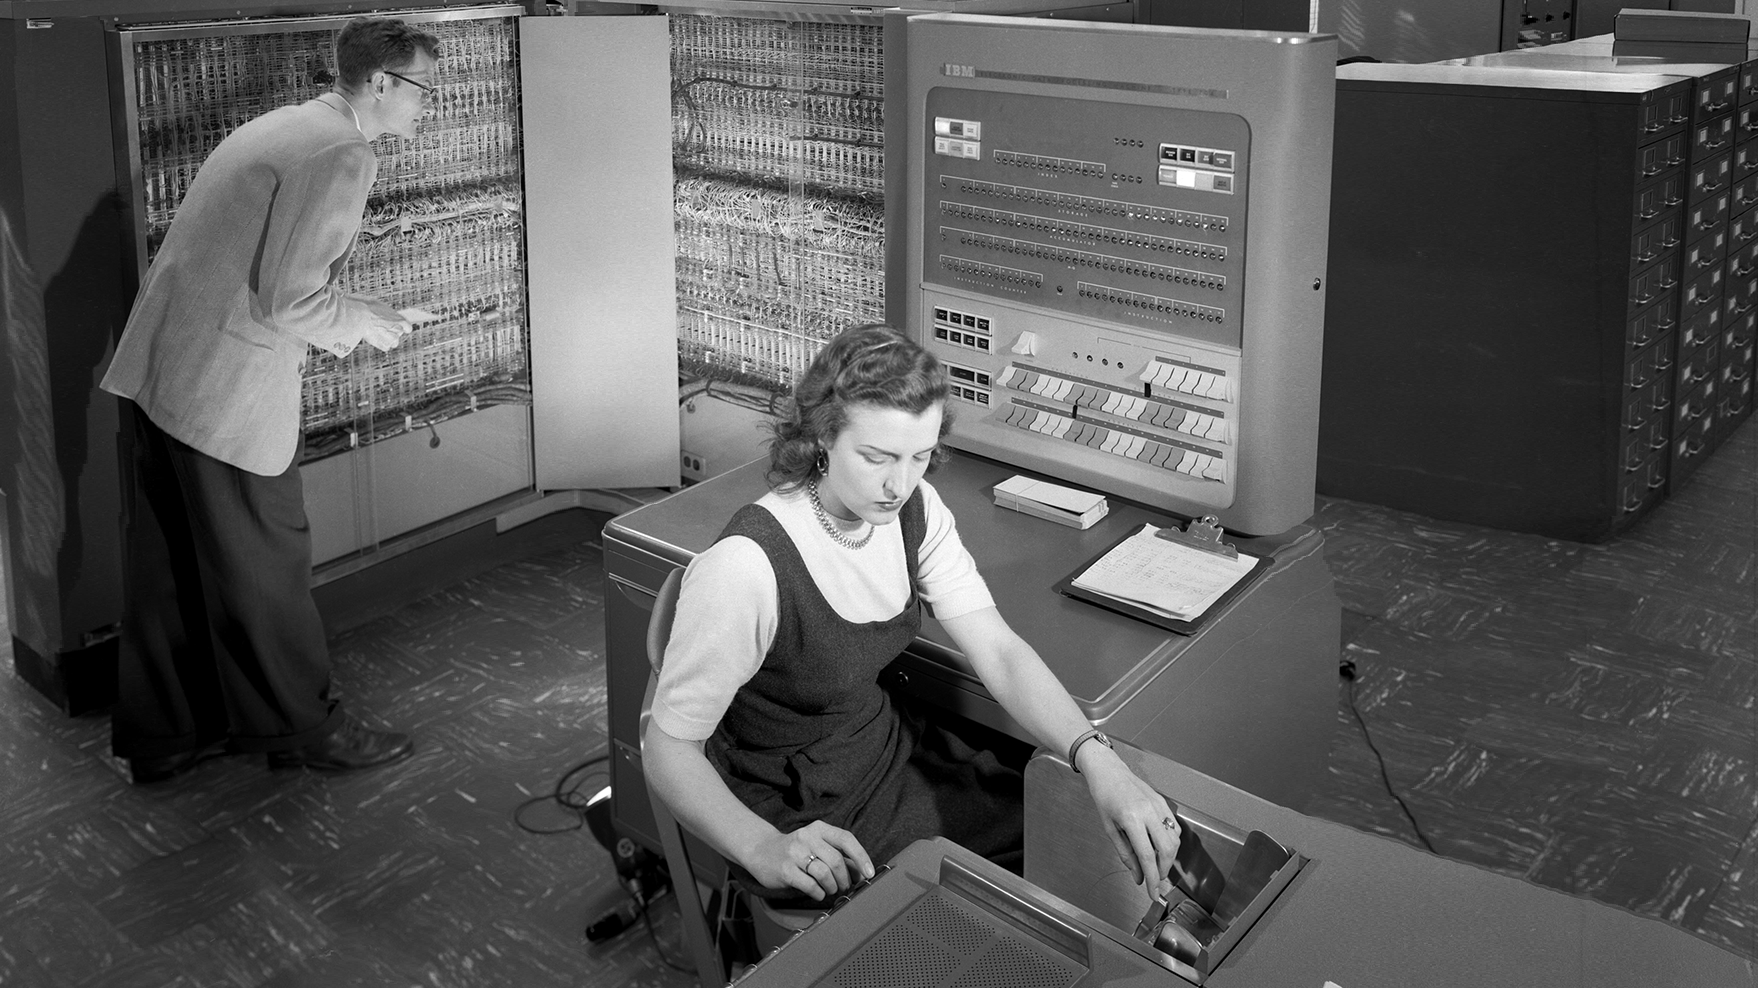
\includegraphics[width=1.05\paperwidth]{Figures/LISP.png}
    }   
}
\begin{frame}[plain]
        %\vskip -20 ex
    %\Large\qquad\qquad\qquad\color{black} {\zA In the beginning there was} \\
    %\Huge LISP
\hfill        {\small\color{white}IBM 704 Computer in 1957}
\vfill\vfill\vfill\vfill\vfill
\begin{minipage}[c]{0.5\textwidth}
        \pause
        \oldBlock{\zA "In the beginning there was":}
        \begin{center}
        \vspace*{2ex}
        \Huge LISP
        \vspace*{1ex}
        \end{center}
        \oldEndBlock
\end{minipage}\hfill


\end{frame}
\setbeamertemplate{background}{}
    \begin{frame}
        \frametitle{LISP}
        \framesubtitle{LISt Processor}
            \begin{center}\texttt{(print "Hello, World!")}\end{center}
        \begin{block}{LISP}
            \begin{itemize}
                \item created in 1958
                \item is the second-oldest high-level programming language in widespread use today
            \end{itemize}
        \end{block}

    \end{frame}
    \begin{frame}[fragile]
        \frametitle{LISP}
        \framesubtitle{LISt Processor}
\begin{minipage}{0.42\textwidth}
\raggedright
LISP is a powerful, but in my opinion, somewhat special language. Here is an example\footnotemark calculating the factorial of a number {\small (directly from Wikipedia)}:
\begin{lstlisting}
(defun factorial (n)
    (if (= n 0) 1
        (* n (factorial (- n 1)))))
\end{lstlisting}
\end{minipage}
\hfill\pause
\begin{minipage}{0.55\textwidth}
\centering
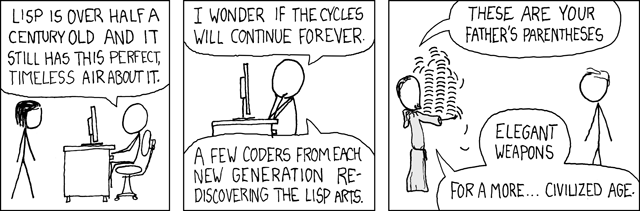
\includegraphics[width=1\textwidth]{Figures/lisp_cycles.png}
\small \texttt{https://xkcd.com/297/}
\end{minipage}
\footnotetext{You do \alert{\underline{not}} need to learn LISP in this course}
    \end{frame}

    \subsection{Map and Reduce}

    \begin{frame}
        \frametitle{Map and Reduce}
        \color{lightgray}
        \begin{center}
            \only<1->{\only<1>{\color{black}}So, why do I talk so much about LISP?}
        \end{center}
        \begin{center}
            \only<2->{\only<2>{\color{black}}It's because its list-based structure had \texttt{map} and \texttt{reduce}}
        \end{center}
        \begin{center}
            \only<3->{\only<3>{\color{black}}Which gave rise to the MapReduce programming model}
        \end{center}
        \begin{center}
            \only<4->{\only<4>{\color{black}}but first, let's talk about \texttt{map} and \texttt{reduce}\ldots}
        \end{center}
    \end{frame}

    \begin{frame}[fragile]
        \frametitle{Map and Reduce}
        \framesubtitle{Map}

            \begin{block}{Map}
                \texttt{map} is a higher-order function that applies a given
                function to each element of, \textit{e.g.}, a list. It can also
                be called \texttt{apply-to-all}.
            \end{block}
            
            \begin{block}{Example: \hfill \small(Python)}
            \begin{center}
            \begin{minipage}{0.8\linewidth}
            \begin{lstlisting}
square = lambda x:x*x
a = [1,2,3,4]
list(map(square, a))
            \end{lstlisting}
            $\Rightarrow$ \texttt{[1, 4, 9, 16]}
            \end{minipage}
            \end{center}
            \end{block}

        
        
    \end{frame}
    
    \begin{frame}[fragile]
        \frametitle{Map and Reduce}
        \framesubtitle{Reduce}

            \begin{block}{Reduce}
                \texttt{reduce} is a higher-order function that by using a
                given function combines the part of, \textit{e.g.}, a list into
                a return value.
            \end{block}

            \begin{block}{Example: \hfill \small(Python)}
            \begin{center}
            \begin{minipage}{0.8\linewidth}
            \begin{lstlisting}
from functools import reduce
sum = lambda a,b:a+b
a = [1,2,3,4]
reduce(sum,a)
            \end{lstlisting}
            $\Rightarrow$ 10
            \end{minipage}
            \end{center}
            \end{block}
    \end{frame}

    \subsection{MapReduce}
    \begin{frame}
        \frametitle{MapReduce}
        \framesubtitle{}
        
    \end{frame}


\section{Spark}
    
    \subsection{Architecture}
    \subsection{RDD}
    \subsection{Dataframe}
\section{Example}
    
\setbeamertemplate{background}{%
    \parbox[c][\paperheight]{\paperwidth}{%
        \vskip -8 ex \hskip -2 em
        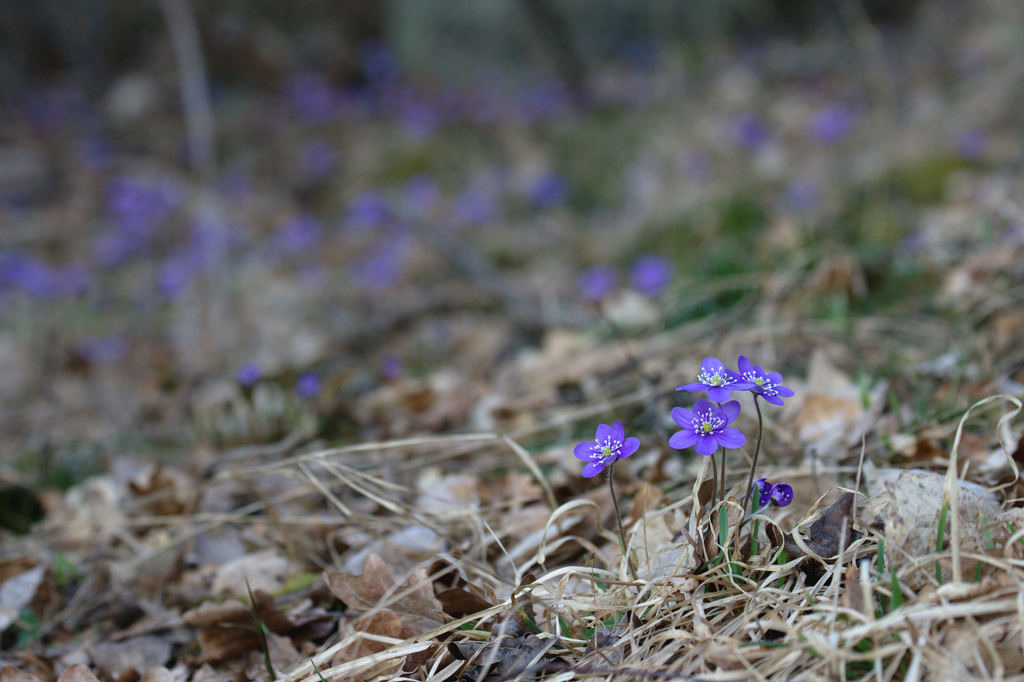
\includegraphics[height=1.5\paperheight]{Figures/blasippa.jpg}
    }   
}
\begin{frame}[plain]
    \vfill\hfill{\Huge\qquad\color{white} \zB Thank \zC you}\hfill\hfill\hfill\vfill
\end{frame}
\setbeamertemplate{background}{}
\end{document}
